% ============================================================
% Plan de Expansion HPTU — Sede Ambulatoria
% Presentacion Abril 2026
% ~35 slides · Narrativa en 6 actos
% Compilar con: lualatex hptu-expansion-abril.tex
% ============================================================
\documentclass[aspectratio=169, 11pt]{beamer}

% -- Tema --
\usetheme{default}
\usecolortheme{default}
\setbeamertemplate{navigation symbols}{}
\setbeamertemplate{footline}{%
  \hspace{8pt}\raisebox{3pt}{
\includegraphics[height=12pt]{basica.png}}%
  \hfill\insertframenumber\,/\,\inserttotalframenumber\hspace{8pt}\vspace{5pt}%
}

% Paleta HPTU
\definecolor{hptu}{HTML}{00549F}
\definecolor{hptudark}{HTML}{003D75}
\definecolor{teal}{HTML}{0D9488}
\definecolor{coral}{HTML}{EF4444}
\definecolor{amber}{HTML}{F59E0B}
\definecolor{slate}{HTML}{64748B}
\definecolor{bglight}{HTML}{F8FAFC}
\definecolor{green}{HTML}{22C55E}
\definecolor{violet}{HTML}{8B5CF6}
\definecolor{rose}{HTML}{E11D48}

\setbeamercolor{frametitle}{fg=hptu}
\setbeamercolor{title}{fg=white}
\setbeamercolor{subtitle}{fg=white!85}
\setbeamercolor{author}{fg=white!80}
\setbeamercolor{date}{fg=white!70}
\setbeamercolor{normal text}{fg=black!85}
\setbeamercolor{structure}{fg=hptu}
\setbeamercolor{itemize item}{fg=teal}
\setbeamercolor{itemize subitem}{fg=hptu}
\setbeamercolor{block title}{fg=white, bg=hptu}
\setbeamercolor{block body}{bg=bglight}
\setbeamercolor{block title alerted}{fg=white, bg=coral}
\setbeamercolor{block body alerted}{bg=coral!5}
\setbeamercolor{block title example}{fg=white, bg=teal}
\setbeamercolor{block body example}{bg=teal!5}

\setbeamerfont{frametitle}{size=\Large, series=\bfseries}
\setbeamerfont{title}{size=\Huge, series=\bfseries}
\setbeamerfont{subtitle}{size=\large}
\setbeamertemplate{itemize items}[circle]

% -- Paquetes --
\usepackage{fontspec}
\usepackage{booktabs}
\usepackage{tabularx}
\usepackage{colortbl}
\usepackage{graphicx}
\usepackage{tikz}
\usetikzlibrary{calc, positioning, shapes.geometric, arrows.meta, backgrounds}
\usepackage{pgfplots}
\pgfplotsset{compat=1.18}
\usepackage{multicol}
\usepackage{hyperref}

% Fuentes
\setsansfont{Helvetica Neue}[
  BoldFont={Helvetica Neue Bold},
  ItalicFont={Helvetica Neue Italic},
]

\newcommand{\highlight}[1]{\textcolor{teal}{\textbf{#1}}}
\newcommand{\danger}[1]{\textcolor{coral}{\textbf{#1}}}
\newcommand{\src}[1]{\par\vspace{2pt}{\tiny\textcolor{slate}{Fuente: #1}}}

% -- Metadata --
\title{Plan de Expansión HPTU}
\subtitle{Sede Ambulatoria --- Localización Estratégica}
\author{Equipo de Análisis Estratégico}
\date{Abril 2026}

\begin{document}

% ============================================================
% ACTO 1: EL PLAN DE EXPANSION (slides 1--4)
% ============================================================

% ---- SLIDE 1: PORTADA ----
{
\setbeamercolor{background canvas}{bg=hptu}
\begin{frame}[plain]
\vfill
\begin{center}
{\usebeamerfont{title}\usebeamercolor[fg]{title}\inserttitle}

\vspace{10pt}
{\usebeamerfont{subtitle}\usebeamercolor[fg]{subtitle}\insertsubtitle}

\vspace{20pt}
\begin{tikzpicture}
  \draw[white, line width=0.5pt] (0,0) -- (8,0);
\end{tikzpicture}

\vspace{14pt}
{\small\textcolor{white!80}{
MCDA 5 dimensiones $\cdot$ 3.8M+ registros $\cdot$ 15 fuentes oficiales}}

\vspace{6pt}
{\small\textcolor{white!60}{
6 zonas evaluadas $\cdot$ Foco ambulatorio $\cdot$ Sin urgencias, sin alta complejidad}}

\vspace{6pt}
{\small\textcolor{white!50}{
Actualizado con feedback de Junta Directiva --- 16 de marzo}}

\vspace{20pt}
{\footnotesize\usebeamercolor[fg]{author}Junta Directiva $\cdot$ \insertdate}
\end{center}
\begin{tikzpicture}[remember picture, overlay]
  \node[anchor=south]
    at ([yshift=14pt]current page.south) {
    
\includegraphics[height=1.2cm]{basica-white.png}
  };
\end{tikzpicture}
\vfill
\end{frame}
}

% ---- SLIDE 2: AGENDA ----
\begin{frame}{Agenda --- 1 hora, 6 actos}

\vspace{4pt}
\begin{center}
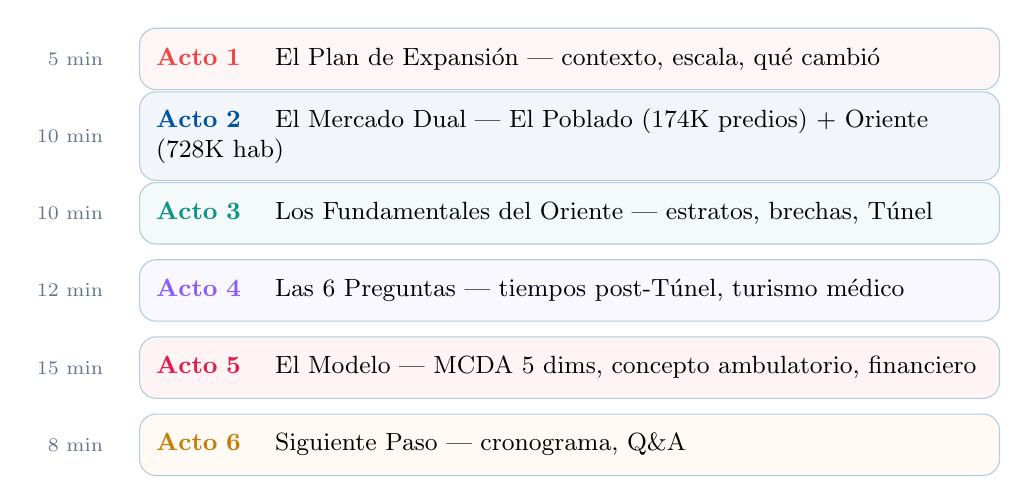
\begin{tikzpicture}[
  act/.style={draw=hptu!30, fill=white, rounded corners=6pt,
              text width=10.5cm, minimum height=0.78cm, align=left,
              font=\small, inner sep=6pt},
  time/.style={font=\scriptsize\color{slate}, anchor=east},
]
\node[act, fill=coral!5] (a1) at (0,0) {
  \textcolor{coral}{\textbf{Acto 1}} \quad El Plan de Expansión --- contexto, escala, qué cambió
};
\node[time] at (-5.8,0) {5 min};

\node[act, fill=hptu!5] (a2) at (0,-0.98) {
  \textcolor{hptu}{\textbf{Acto 2}} \quad El Mercado Dual --- El Poblado (174K predios) + Oriente (728K hab)
};
\node[time] at (-5.8,-0.98) {10 min};

\node[act, fill=teal!5] (a3) at (0,-1.96) {
  \textcolor{teal}{\textbf{Acto 3}} \quad Los Fundamentales del Oriente --- estratos, brechas, Túnel
};
\node[time] at (-5.8,-1.96) {10 min};

\node[act, fill=violet!5] (a4) at (0,-2.94) {
  \textcolor{violet}{\textbf{Acto 4}} \quad Las 6 Preguntas --- tiempos post-Túnel, turismo médico
};
\node[time] at (-5.8,-2.94) {12 min};

\node[act, fill=rose!5] (a5) at (0,-3.92) {
  \textcolor{rose}{\textbf{Acto 5}} \quad El Modelo --- MCDA 5 dims, concepto ambulatorio, financiero
};
\node[time] at (-5.8,-3.92) {15 min};

\node[act, fill=amber!5] (a6) at (0,-4.9) {
  \textcolor{amber!80!black}{\textbf{Acto 6}} \quad Siguiente Paso --- cronograma, Q\&A
};
\node[time] at (-5.8,-4.9) {8 min};
\end{tikzpicture}
\end{center}

\vspace{4pt}
{\footnotesize\textcolor{slate}{Dashboard interactivo: \url{https://hptu-localizacion.vercel.app}}}
\end{frame}

% ---- SLIDE 3: QUE CAMBIO (resumen visual) ----
\begin{frame}{Lo que cambió desde la Junta del 16 de marzo}

\begin{columns}[T]
\column{0.48\textwidth}
\begin{alertblock}{\small Feedback de la Junta}
\footnotesize
\begin{enumerate}\setlength{\itemsep}{2pt}
  \item \textbf{Nombre:} ``Nueva Sede'' $\to$ \highlight{Plan de Expansión}
  \item \textbf{Foco:} Ambulatorio, \danger{sin urgencias ni alta complejidad}
  \item \textbf{SVF:} Faltaba en tabla --- es \highlight{duopolio Somer + SVF}
  \item \textbf{MCDA:} Reemplazar ``Valor Inmobiliario'' con \highlight{Visibilidad + Esperas Productivas}
  \item \textbf{Estratos:} ¿Cuántos son E4/5/6 de los 728K?
  \item \textbf{Conceptos:} Cleveland Clinic, PRENUVO, wellness
\end{enumerate}
\end{alertblock}

\column{0.48\textwidth}
\begin{exampleblock}{\small Lo que se hizo}
\footnotesize
\begin{itemize}\setlength{\itemsep}{2pt}
  \item[$\checkmark$] \textbf{5 dimensiones MCDA} (Acc 30\%, Dem 25\%, Comp 20\%, Vis 15\%, Esp 10\%)
  \item[$\checkmark$] SVF en todas las tablas de brechas
  \item[$\checkmark$] Proxy estratos Oriente (Decreto 096/2021 Rionegro)
  \item[$\checkmark$] Portafolio ambulatorio (7 categorías, sin urgencias/UCI)
  \item[$\checkmark$] Modelo financiero ambulatorio (\$67,000M)
  \item[$\checkmark$] Tiempos post-Túnel 2da etapa
  \item[$\checkmark$] Referentes: Cleveland Clinic, PRENUVO, CEDIMED
\end{itemize}
\end{exampleblock}
\end{columns}
\end{frame}

% ---- SLIDE 3b: QUE CAMBIO (narrativa detallada) ----
\begin{frame}{Los seis ajustes, en detalle}

\begin{columns}[T]
\column{0.48\textwidth}
\scriptsize
\begin{enumerate}\setlength{\itemsep}{4pt}
  \item \textbf{Nombre $\to$ Plan de Expansión.} Esto no es un hospital nuevo. Es la expansión ambulatoria de HPTU --- herencia de marca, mismos protocolos, mismos especialistas.

  \item \textbf{Foco ambulatorio.} Siete categorías de servicio: imágenes, consulta, cirugía de día, chequeo ejecutivo, rehabilitación, estética y oncología ambulatoria. \danger{Cero camas, cero urgencias, cero UCI.}

  \item \textbf{Duopolio Somer + SVF.} San Vicente Fundación Rionegro tiene oncología, radioterapia, cirugía y pediatría subespecializada. Toda la presentación refleja que es un \highlight{duopolio}. Nuestra propuesta ambulatoria \textbf{complementa} a ambos, no compite.
\end{enumerate}

\column{0.48\textwidth}
\scriptsize
\begin{enumerate}\setcounter{enumi}{3}\setlength{\itemsep}{4pt}
  \item \textbf{MCDA: Visibilidad + Esperas Productivas.} No compramos terreno --- arrendamos en Access Point. El valor inmobiliario es irrelevante. Lo que importa: cuánta gente nos ve (\highlight{42K veh/día}) y qué ecosistema hay alrededor.

  \item \textbf{Estratos Oriente.} Solo Rionegro tiene dato directo (Decreto 096/2021): \highlight{42\%} de viviendas son E4+. Para los demás municipios: proxy conservador basado en afiliación contributiva. Somos transparentes sobre las limitaciones.

  \item \textbf{Referentes internacionales.} Cleveland Clinic: 270 centros ambulatorios satélite. PRENUVO: MRI preventivo como diferenciador premium. CEDIMED: valida el modelo de imágenes pero no tiene presencia en el Oriente.
\end{enumerate}
\end{columns}
\end{frame}

% ---- SLIDE 4: ESCALA DEL ANALISIS ----
\begin{frame}{La escala del análisis}

\begin{columns}[T]
\column{0.48\textwidth}
\begin{block}{\small Datos procesados}
\scriptsize
\begin{tabular}{@{}lr@{}}
\toprule
Fuentes primarias & \textbf{15} \\
Registros procesados & \textbf{3.8M+} \\
Zonas evaluadas & \textbf{6} \\
Dimensiones MCDA & \textbf{5} \\
Competidores perfilados & \textbf{13} \\
Barrios analizados & \textbf{22} \\
Municipios Oriente & \textbf{11} \\
Periodo de datos & 2017--2037 \\
\bottomrule
\end{tabular}
\end{block}

\column{0.48\textwidth}
\begin{exampleblock}{\small Modelo MCDA (score 0--100)}
\scriptsize
5 dimensiones, pesos confirmados post-Junta:

\vspace{3pt}
$\text{Score} = \underbrace{A \times 30\%}_{\text{Acc.}} + \underbrace{D \times 25\%}_{\text{Dem.}} + \underbrace{C \times 20\%}_{\text{Comp.}} + \underbrace{\text{Vis} \times 15\%}_{\text{Visib.}} + \underbrace{\text{Esp} \times 10\%}_{\text{Esperas}}$

\vspace{4pt}
\textbf{Nuevas variables:}\\
$\bullet$ \textbf{Visibilidad:} tráfico vehicular, exposición\\
$\bullet$ \textbf{Esperas Productivas:} retail/servicios en 500m

\vspace{3pt}
Validado con \textbf{Monte Carlo} (3,000 iter., 6 escenarios).
\end{exampleblock}
\end{columns}

\src{Catastro, REPS, MEData Aforos, DANE, POT, ANI, Mapbox, Google Places, OSM}
\end{frame}

% ============================================================
% ACTO 2: EL MERCADO DUAL (slides 5--10)
% ============================================================

% ---- MEDELLIN METROPOLITANO ----
\begin{frame}{Medellín Metropolitano: el mercado principal}

\begin{columns}[T]
\column{0.48\textwidth}
\vspace{-2pt}
{\scriptsize\setlength{\tabcolsep}{3pt}
\begin{tabular}{@{}lrrr@{}}
\toprule
\textbf{Municipio} & \textbf{2018} & \textbf{2026} & \textbf{Crec.} \\
\midrule
\rowcolor{teal!8}
Medellín & 2,327,880 & 2,471,274 & +6.1\% \\
\rowcolor{teal!6}
Envigado & 210,705 & 246,874 & +17.1\% \\
Itagüí & 240,828 & 256,679 & +6.6\% \\
\rowcolor{teal!6}
Sabaneta & 73,838 & 87,879 & \highlight{+19.0\%} \\
\midrule
\textbf{Total metro} & \textbf{2,853,251} & \textbf{3,062,706} & +7.3\% \\
\midrule
\rowcolor{hptu!5}
El Poblado & 134,873 & 163,578 & +21.2\% \\
\bottomrule
\end{tabular}
}

\vspace{3pt}
\src{DANE CNPV 2018, DENSURBAM proyecciones tendenciales}

\column{0.49\textwidth}
\begin{exampleblock}{\small El mercado premium}
\footnotesize
\begin{tabular}{@{}lr@{}}
Predios E5/E6 corredor & \highlight{174,543} \\
Predios E6 (El Poblado) & 38,415 \\
Avalúo promedio E6 & \$437.8M COP \\
Afiliados prepagada SURA & 320,000 \\
Prepagada Antioquia & \highlight{1.4M afiliados} \\
Revenue prepagada/año & \highlight{COP \$7,2 billones} \\
Crecimiento 2022-25 & +37\% \\
\end{tabular}
\end{exampleblock}

\vspace{2pt}
\begin{alertblock}{\small Proyección 2037}
\centering\footnotesize
Valle de Aburrá: \textbf{+152K personas}\\
El Poblado: \textbf{180,314 hab} (+20.6\%)\\
Sabaneta: +19.0\% · Envigado: +17.1\%
\end{alertblock}
\end{columns}
\end{frame}

% ---- DEFICIT DE SALUD MEDELLIN ----
{
\setbeamercolor{background canvas}{bg=coral!3}
\begin{frame}{Déficit de salud: 0.54 camas por 1,000 habitantes}

\begin{columns}[T]
\column{0.48\textwidth}
\vspace{-2pt}
{\scriptsize
\begin{tabular}{@{}lccc@{}}
\toprule
\textbf{Municipio} & \textbf{Camas/1000} & \textbf{OMS mín.} & \textbf{Déficit} \\
\midrule
\rowcolor{coral!10}
Medellín & \danger{1.0} & 3.0 & --67\% \\
\rowcolor{coral!10}
Envigado & \danger{0.6} & 3.0 & --80\% \\
\rowcolor{coral!10}
Itagüí & \danger{0.6} & 3.0 & --80\% \\
\rowcolor{coral!10}
Sabaneta & \danger{0.5} & 3.0 & --83\% \\
\midrule
\textbf{Corredor Las Palmas} & \danger{0.0} & 3.0 & \danger{--100\%} \\
\bottomrule
\end{tabular}
}

\vspace{4pt}
\begin{block}{\small DENSURBAM confirma}
\scriptsize
IRS Salud El Poblado: \danger{0.27} (umbral: 2.5)\\
\textbf{5 veces por debajo} del mínimo de sostenibilidad.\\
\textbf{10 barrios} con \danger{0.0 m²} de oferta de salud.
\end{block}

\column{0.49\textwidth}
\begin{alertblock}{\small Corredor Las Palmas al 2037}
\footnotesize
\begin{tabular}{@{}lr@{}}
Habitantes sin cobertura & \danger{103,913} \\
Oferta actual (m²/hab) & \danger{0.0} \\
Estándar requerido & 3.5 m²/hab \\
\midrule
\textbf{m² equipamiento necesario} & \danger{363,696} \\
\end{tabular}

\vspace{3pt}
{\scriptsize Con crecimiento de \textbf{+20.6\%} al 2037, la brecha solo se ampliará. \highlight{La sede ambulatoria HPTU cerraría directamente este déficit.}}
\end{alertblock}

\vspace{2pt}
\begin{exampleblock}{\small Hospitales más cercanos al corredor}
\tiny
\begin{tabular}{@{}lrl@{}}
Cl.\ Rosario Tesoro & 158 camas & \highlight{0.93 km} \\
Cl.\ Las Vegas & 171 camas & 3.12 km \\
Cl.\ CES & 213 camas & 7.16 km \\
\midrule
& & \danger{Sin alta complej.} \\
\end{tabular}
\end{exampleblock}
\end{columns}

\src{REPS (s2ru-bqt6), DENSURBAM (URBAM-EAFIT/AMVA), DANE proyecciones}
\end{frame}
}

% ---- SLIDE 5: EL POBLADO ----
\begin{frame}{Mercado 1: El Poblado --- 174,543 predios E5/E6}

\begin{columns}[T]
\column{0.46\textwidth}
{\scriptsize\setlength{\tabcolsep}{3pt}
\begin{tabular}{@{}lrrc@{}}
\toprule
\textbf{Barrio} & \textbf{E5/E6} & \textbf{\%} & \textbf{Avalúo} \\
\midrule
\rowcolor{teal!8}
\textbf{El Poblado core} & \textbf{38,415} & \textbf{98} & \$371M \\
Castropol & 6,228 & 97 & \$327M \\
Los Balsos No.\ 1 & 4,019 & 95 & \$401M \\
San Lucas & 3,671 & 93 & \$512M \\
Manila & 2,144 & 96 & \$305M \\
\rowcolor{teal!6}
Altos del Poblado & 1,867 & 91 & \$245M \\
{\tiny + 15 barrios más} & & & \\
\midrule
\textbf{Total 22 barrios} & \textbf{174,543} & & \\
\bottomrule
\end{tabular}
}

\vspace{4pt}
\src{Catastro Medellín (bp59-rj8r)}

\column{0.50\textwidth}
\begin{exampleblock}{\small Corredor Las Palmas}
\footnotesize
\begin{itemize}\setlength{\itemsep}{2pt}
  \item \highlight{42,000 veh/día} en Av.\ Las Palmas (MEData)
  \item \danger{0 camas} de alta complejidad en el corredor
  \item POT permite hasta \highlight{19 pisos} en San Lucas
  \item Solo \highlight{45.8\%} de densidad usada
  \item 103,913 hab.\ sin cobertura a 2037 (DENSURBAM)
\end{itemize}
\end{exampleblock}

\vspace{4pt}
\begin{alertblock}{\small Brecha}
\centering\footnotesize
\textbf{174K predios E5/E6\\a $>$20 min de HPTU Robledo}
\end{alertblock}
\end{columns}
\end{frame}

% ---- SLIDE 6: ORIENTE ----
\begin{frame}{Mercado 2: Oriente Antioqueño --- 728,000 habitantes}

\begin{columns}[T]
\column{0.48\textwidth}
{\scriptsize\setlength{\tabcolsep}{3pt}
\begin{tabular}{@{}lrr@{}}
\toprule
\textbf{Municipio} & \textbf{Pob.\ 2018} & \textbf{\% Contrib.} \\
\midrule
\rowcolor{teal!8}
Rionegro & 116,400 & \highlight{54.9\%} \\
Marinilla & 56,399 & 41.1\% \\
\rowcolor{teal!6}
La Ceja & 53,134 & \highlight{51.4\%} \\
Guarne & 52,570 & 42.9\% \\
El Carmen & 48,988 & 31.5\% \\
\rowcolor{teal!6}
El Retiro & 19,695 & \highlight{56.8\%} \\
{\scriptsize + 5 municipios} & & \\
\midrule
\textbf{Total Oriente} & \textbf{728,581} & \textbf{42.8\%} \\
\bottomrule
\end{tabular}
}

\vspace{3pt}
\src{DANE CNPV 2018, RUAF Aseguramiento}

\column{0.49\textwidth}
\begin{alertblock}{\small Infraestructura de salud: duopolio}
\footnotesize
Alta complejidad en Oriente:
\begin{itemize}\setlength{\itemsep}{1pt}
  \item \textbf{Cl.\ Somer} --- oncología (UFCA), radioterapia, trasplante cardíaco
  \item \textbf{SVF Rionegro} --- oncología, cirugía, pediatría sub., va a 500 camas
\end{itemize}
\vspace{3pt}
\danger{Duopolio}, no monopolio.\\
\highlight{Oportunidad: ambulatorio especializado} que complementa, no compite.
\end{alertblock}

\vspace{4pt}
{\scriptsize\textbf{Crecimiento:} +1.64\%/año, migración 5.2/100 hab, PIB 10.4\% de Antioquia}
\end{columns}
\end{frame}

% ---- SLIDE 7: ESTRATOS ORIENTE ----
{
\setbeamercolor{background canvas}{bg=amber!3}
\begin{frame}{Dato faltante: ¿Cuántos son estrato 4/5/6 en el Oriente?}

\begin{columns}[T]
\column{0.50\textwidth}
\begin{alertblock}{\small Dato directo: solo Rionegro}
\scriptsize
\begin{tabular}{@{}lrr@{}}
\toprule
\textbf{Estrato} & \textbf{Viviendas} & \textbf{\%} \\
\midrule
E1 & 1,879 & 4.2\% \\
E2 & 7,221 & 16.1\% \\
E3 & 16,853 & 37.6\% \\
\rowcolor{teal!10}
\textbf{E4} & \textbf{15,633} & \textbf{34.9\%} \\
\rowcolor{teal!8}
E5 & 2,723 & 6.1\% \\
\rowcolor{teal!6}
E6 & 496 & 1.1\% \\
\midrule
\textbf{Total} & \textbf{44,805} & \\
\rowcolor{teal!12}
\textbf{E4+} & \textbf{18,852} & \textbf{42.1\%} \\
\bottomrule
\end{tabular}

\vspace{3pt}
{\tiny Fuente: Decreto 096/2021 Rionegro, DiariOriente}
\end{alertblock}

\column{0.47\textwidth}
\begin{block}{\small Proxy para otros municipios}
\footnotesize
No existe dataset directo en datos.gov.co.

\vspace{3pt}
\textbf{Método:} ratio E4+/contributivo de Rionegro (0.765) aplicado a \% contributivo de cada municipio.

\vspace{4pt}
\scriptsize
\begin{tabular}{@{}lr@{}}
\toprule
\textbf{Municipio} & \textbf{E4+ est.} \\
\midrule
\textbf{Rionegro} (directo) & \highlight{18,852} \\
La Ceja & 7,222 \\
Marinilla & 6,143 \\
Guarne & 5,929 \\
El Carmen & 4,078 \\
El Retiro & 2,909 \\
{\tiny + 5 municipios} & \\
\midrule
\textbf{Total Oriente} & \highlight{$\sim$53,800} \\
\bottomrule
\end{tabular}
\end{block}
\end{columns}

\vspace{2pt}
{\tiny\textcolor{amber!80!black}{\textbf{Transparencia:}} estimación conservadora. Solo Rionegro tiene dato directo. Proxy asume relación estrato-régimen similar entre municipios.}
\end{frame}
}

% ---- SLIDE 8: BRECHAS AMBULATORIAS ----
\begin{frame}{Brechas ambulatorias en el Oriente (actualizado con SVF)}
\vspace{-4pt}
{\scriptsize\setlength{\tabcolsep}{4pt}
\begin{tabular}{@{}p{3.5cm}p{3.5cm}cp{4.5cm}@{}}
\toprule
\textbf{Servicio} & \textbf{Status Oriente} & \textbf{Nivel} & \textbf{Oportunidad HPTU} \\
\midrule
\rowcolor{coral!8}
Cirugía Ambulatoria & Campestre + SVF (limitada) & Limitado & Hub quirúrgico: ortop., urología, ORL \\
Imágenes Avanzadas & IMEDI + Somer (limitado) & Limitado & Centro TAC, RMN, PET-CT (Fase 2), PRENUVO \\
\rowcolor{coral!8}
Oncología Ambulatoria & Somer y SVF (duopolio) & Limitado & QT ambulatoria, 2da opinión \\
Radioterapia & Somer y SVF (duopolio) & Limitado & 3er centro si demanda lo justifica \\
\rowcolor{coral!8}
Rehabilitación Esp. & Básica únicamente & \danger{Inexist.} & Neuro, cardíaca, deportiva \\
Chequeo Ejecutivo & Inexistente & \danger{Inexist.} & Premium: Zona Franca + aeropuerto \\
\rowcolor{coral!8}
Turismo Médico & SVF (incipiente) & Limitado & 23,323 pac int./año, cerca aeropuerto \\
Pediatría Sub. & SVF Rionegro (limitada) & Limitado & Ampliar cobertura ambulatoria \\
\bottomrule
\end{tabular}
}

\vspace{2pt}
\begin{columns}[T]
\column{0.50\textwidth}
\begin{exampleblock}{\small Corrección post-Junta}
\scriptsize
\textbf{SVF Rionegro tiene:} oncología, radioterapia, cirugía amb., pediatría sub., turismo médico. Es \highlight{duopolio Somer + SVF}.
\end{exampleblock}
\column{0.46\textwidth}
\begin{alertblock}{\small Oportunidad HPTU}
\scriptsize
Sede ambulatoria \textbf{no compite} con Somer ni SVF en alta complejidad. \highlight{Complementa} con servicios que hoy requieren referencia a Medellín.
\end{alertblock}
\end{columns}
\src{REPS (b4dp-ximh), Google Places, Junta Directiva 16 marzo}
\end{frame}

% ---- SLIDE 9: TRAFICO ----
\begin{frame}{42,000 vehículos/día en Vía Las Palmas}
\begin{columns}[T]
\column{0.50\textwidth}
{\scriptsize\textbf{Corredores de acceso al Oriente:}}

\vspace{2pt}
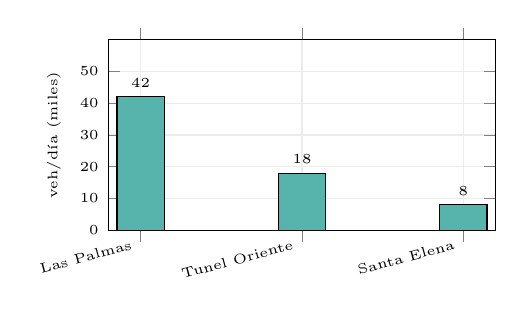
\begin{tikzpicture}
\begin{axis}[
  ybar, width=6.5cm, height=4cm,
  bar width=0.6cm,
  symbolic x coords={Las Palmas, Tunel Oriente, Santa Elena},
  xtick=data,
  xticklabel style={font=\tiny, rotate=15, anchor=east},
  ylabel={\tiny veh/día (miles)},
  ymin=0, ymax=60,
  ytick={0,10,20,30,40,50},
  yticklabel style={font=\tiny},
  nodes near coords,
  every node near coord/.append style={font=\tiny\bfseries},
  grid=major, grid style={gray!15},
]
\addplot[fill=teal!70] coordinates {(Las Palmas,42) (Tunel Oriente,18) (Santa Elena,8)};
\end{axis}
\end{tikzpicture}
\src{MEData Aforos (b9s9-jw7c), 64,285 obs.}

\column{0.47\textwidth}
\begin{exampleblock}{\small Access Point = máxima visibilidad}
\scriptsize
\begin{itemize}\setlength{\itemsep}{1pt}
  \item Km 7 Vía Las Palmas, Retorno 5
  \item \highlight{Todo vehículo al Túnel pasa por Km 7}
  \item Sin pico y placa
  \item 2da etapa Túnel (H2 2027): \highlight{tráfico se duplica}
  \item Score Visibilidad: \highlight{78/100}
\end{itemize}
\end{exampleblock}

\vspace{2pt}
\begin{block}{\small Velocidad por hora}
\scriptsize
\begin{tabular}{@{}lcc@{}}
\toprule
& Las Palmas & Poblado \\
\midrule
AM (8:00) & 40.9 km/h & 22.5 km/h \\
\rowcolor{coral!8}
PM (17:00) & 36.1 km/h & \danger{18.0 km/h} \\
\bottomrule
\end{tabular}
\end{block}
\end{columns}
\vspace{1pt}
{\tiny\textcolor{amber!80!black}{\textbf{Nota:}} Tráfico genera reconocimiento de marca. Demanda médica se genera por referencia médica y contratos EPS.}
\end{frame}

% ---- SLIDE 10: TUNEL 2DA ETAPA ----
{
\setbeamercolor{background canvas}{bg=teal!3}
\begin{frame}{2da Etapa Túnel de Oriente: el game changer (H2 2027)}
\begin{columns}[T]
\column{0.48\textwidth}
\begin{block}{\small El proyecto}
\scriptsize
\begin{tabular}{@{}lr@{}}
Inversión & COP \$1.8 billones \\
Avance & 19\% (mar 2026) \\
Túnel Santa Elena 2 & 8.2 km excavado \\
Entrega & H2 2027 \\
Impacto & Doble calzada completa \\
\end{tabular}

\vspace{2pt}
Access Point en Km 7 = \highlight{nodo de entrada} a la doble calzada.
\end{block}

\vspace{2pt}
\begin{alertblock}{\small Impacto en tiempos de viaje}
\scriptsize
\begin{tabular}{@{}lcc@{}}
\toprule
\textbf{Destino} & \textbf{Hoy} & \textbf{Post-Túnel} \\
\midrule
\rowcolor{teal!10}
Aeropuerto SKRG & 51 min & \highlight{$\sim$25 min} \\
El Retiro & 44 min & \highlight{$\sim$28 min} \\
Rionegro & 59 min & $\sim$38 min \\
Marinilla & 67 min & $\sim$43 min \\
La Ceja & 65 min & $\sim$42 min \\
\bottomrule
\end{tabular}
\end{alertblock}

\column{0.49\textwidth}
\begin{exampleblock}{\small Infraestructura complementaria}
\scriptsize
\begin{itemize}\setlength{\itemsep}{1pt}
  \item \textbf{Intercambio Alto Palmas} (\$18,000M) --- elimina congestión
  \item \textbf{Vía Aeropuerto-Belén} (\$120,000M) --- acorta 12 km
  \item \textbf{Vía Llanogrande-Cañada} (\$120,000M) --- La Ceja a 10 min
  \item \textbf{Tren Ligero Rionegro} --- anulado (8-10 años)
\end{itemize}
\end{exampleblock}

\vspace{2pt}
\begin{exampleblock}{\small Aeropuerto JMC: Plan Maestro 2055}
\centering\footnotesize
14.5M $\to$ \highlight{42.7M pasajeros}\\
{\scriptsize COP \$22 billones $\cdot$ A \highlight{$\sim$25 min} de AP post-Túnel}
\end{exampleblock}
\end{columns}
\end{frame}
}

% ============================================================
% ACTO 3: LOS FUNDAMENTALES DEL ORIENTE (slides 11--16)
% ============================================================

% ---- SLIDE 11: INFRAESTRUCTURA DE SALUD ORIENTE ----
{
\setbeamercolor{background canvas}{bg=coral!3}
\begin{frame}{Infraestructura de salud del Oriente: concentrada y crítica}
\begin{columns}[T]
\column{0.48\textwidth}
{\tiny\setlength{\tabcolsep}{3pt}
\begin{tabular}{@{}lrrr@{}}
\toprule
\textbf{Municipio} & \textbf{Camas} & \textbf{/1000} & \textbf{Gap OMS} \\
\midrule
\rowcolor{teal!6}
Rionegro & 656 & 4.86 & --- \\
La Ceja & 240 & 3.48 & --- \\
Guarne & 184 & 3.73 & --- \\
\rowcolor{coral!10}
El Carmen & 37 & \danger{0.59} & +1.91 \\
\rowcolor{coral!10}
Marinilla & 27 & \danger{0.42} & +2.08 \\
\rowcolor{coral!10}
El Retiro & 26 & \danger{1.08} & +1.42 \\
\rowcolor{coral!10}
El Santuario & 6 & \danger{0.17} & +2.33 \\
\midrule
\textbf{Total Oriente} & \textbf{1,199} & & \\
\bottomrule
\end{tabular}
}
\src{REPS capacidad instalada (b4dp-ximh), DANE est.\ 2026}

\column{0.49\textwidth}
\begin{alertblock}{\small 3 datos críticos}
\scriptsize
\begin{enumerate}\setlength{\itemsep}{0pt}
  \item \textbf{55\%} de camas concentradas en Rionegro
  \item \danger{Duopolio Somer + SVF} en alta complejidad
  \item \textbf{4 municipios} con $<$1 cama/1000 hab
\end{enumerate}
\end{alertblock}

\vspace{2pt}
\begin{exampleblock}{\small Oportunidad ambulatoria}
\scriptsize
La brecha no es de camas (Somer y SVF lo cubren). La brecha es de \highlight{servicios ambulatorios especializados}: imágenes, rehabilitación, chequeo ejecutivo, cirugía de día.
\end{exampleblock}
\end{columns}
\end{frame}
}

% ---- SLIDE 12: 8 INDICADORES UP ----
\begin{frame}{8 de 8 indicadores apuntan al Oriente}

\vspace{-2pt}
\begin{center}
{\scriptsize\setlength{\tabcolsep}{4pt}
\begin{tabular}{@{}clcc@{}}
\toprule
\textbf{\#} & \textbf{Indicador} & \textbf{Valor} & \textbf{Tendencia} \\
\midrule
1 & Población Oriente (DANE) & 728,581 & \textcolor{green}{$\uparrow$ +1.64\%/año} \\
\rowcolor{teal!6}
2 & Tráfico Las Palmas (MEData) & 42,000 veh/día & \textcolor{green}{$\uparrow$ +89\% en 10 años} \\
3 & Pasajeros aeropuerto (Aerocivil) & 14.5M $\to$ 42.7M & \textcolor{green}{$\uparrow$ Plan Maestro 2055} \\
\rowcolor{teal!6}
4 & Prepagada Antioquia (SURA) & 1.4M afiliados & \textcolor{green}{$\uparrow$ +37\% (2022-25)} \\
5 & Contributivos Oriente (RUAF) & 384,171 & \textcolor{green}{$\uparrow$ ratio C/S = 3.46$\times$} \\
\rowcolor{teal!6}
6 & Zona Franca empresas & 300 + 12K emp. & \textcolor{green}{$\uparrow$ expansión} \\
7 & Inversión infraestructura vial & COP \$2+ billones & \textcolor{green}{$\uparrow$ 5 proyectos} \\
\rowcolor{teal!6}
8 & Cirugía ambulatoria Colombia & 490,944 proc/año & \textcolor{green}{$\uparrow$ +10\% YoY} \\
\bottomrule
\end{tabular}
}
\end{center}

\vspace{6pt}
\begin{exampleblock}{}
\centering\large
\highlight{8 de 8 indicadores son crecientes.}\\[4pt]
\footnotesize La demanda no va a disminuir.
\end{exampleblock}

\src{DANE, MEData, Aerocivil, SURA, RUAF, MinSalud}
\end{frame}

% ---- SLIDE 12: DEMANDA CAPTURABLE ----
\begin{frame}{Demanda capturable: 45,000 consultas/año desde el Oriente}

\begin{columns}[T]
\column{0.48\textwidth}
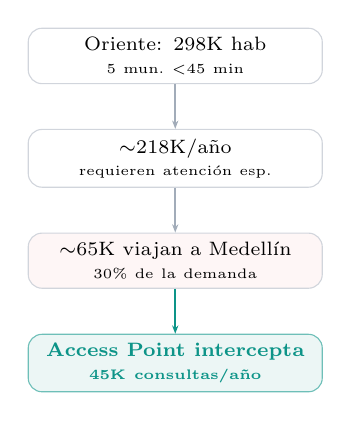
\begin{tikzpicture}[
  box/.style={draw=slate!30, fill=white, rounded corners=5pt,
              text width=3.5cm, minimum height=0.7cm, align=center,
              font=\scriptsize},
  hub/.style={box, draw=teal!60, fill=teal!8, font=\scriptsize\bfseries},
  flow/.style={-{Stealth[length=3pt]}, thick},
]
\node[box] (pop) at (0,0) {Oriente: 298K hab\\{\tiny 5 mun.\ $<$45 min}};
\node[box] (need) at (0,-1.3) {$\sim$218K/año\\{\tiny requieren atención esp.}};
\node[box, fill=coral!5] (med) at (0,-2.6) {$\sim$65K viajan a Medellín\\{\tiny 30\% de la demanda}};
\node[hub] (ap) at (0,-3.9) {\textcolor{teal}{Access Point intercepta}\\{\tiny \highlight{45K consultas/año}}};

\draw[flow, slate!60] (pop) -- (need);
\draw[flow, slate!60] (need) -- (med);
\draw[flow, teal] (med) -- (ap);
\end{tikzpicture}

\column{0.49\textwidth}
\begin{exampleblock}{\small Mercado contributivo por municipio}
\scriptsize
\begin{tabular}{@{}lrc@{}}
\toprule
& \textbf{Contrib.} & \textbf{$>$50\%?} \\
\midrule
\rowcolor{teal!8}
Rionegro & 161,041 & \highlight{Sí} \\
El Retiro & 10,845 & \highlight{Sí} \\
\rowcolor{teal!6}
La Ceja & 26,920 & \highlight{Sí} \\
Guarne & 22,100 & No \\
Marinilla & 22,900 & No \\
\midrule
\textbf{Total} & \textbf{384,171} & \\
\bottomrule
\end{tabular}
\end{exampleblock}

\vspace{4pt}
{\scriptsize 3 municipios con $>$50\% contributivo = \textbf{mercado privado fuerte}. SURA domina 64-79\%.}
\end{columns}

\src{BDUA marzo 2026 (ADRES), RUAF Aseguramiento}
\end{frame}

% ============================================================
% ACTO 4: LAS 6 PREGUNTAS (slides 13--18)
% ============================================================

% ---- SLIDE 13: RESUMEN 6 PREGUNTAS ----
{
\setbeamercolor{background canvas}{bg=teal!3}
\begin{frame}{6 preguntas, 6 respuestas: todas Sí}

\begin{center}
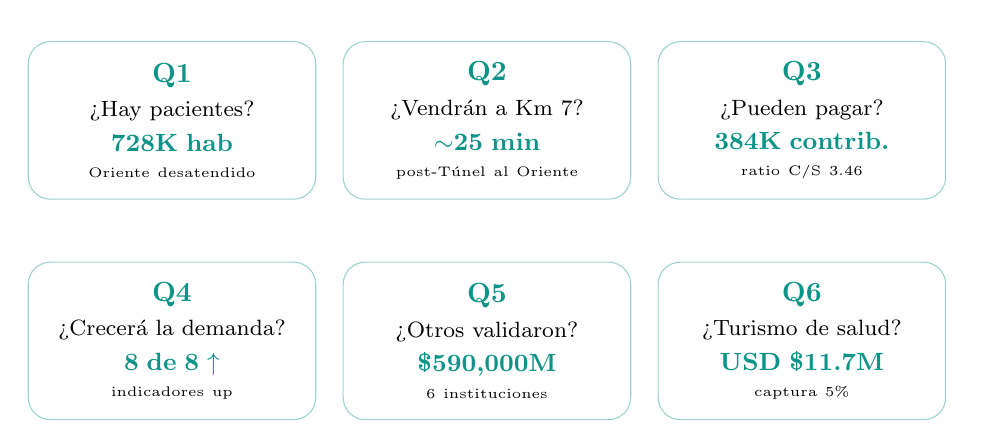
\begin{tikzpicture}[
  qbox/.style={draw=teal!40, fill=white, rounded corners=8pt,
               text width=3.3cm, minimum height=2.0cm, align=center,
               font=\footnotesize, inner sep=5pt},
]
\node[qbox] (q1) at (0,0) {
  {\normalsize\textcolor{teal}{\textbf{Q1}}}\\[3pt]
  ¿Hay pacientes?\\[3pt]
  {\small\highlight{728K hab}}\\{\tiny Oriente desatendido}
};
\node[qbox] (q2) at (4,0) {
  {\normalsize\textcolor{teal}{\textbf{Q2}}}\\[3pt]
  ¿Vendrán a Km 7?\\[3pt]
  {\small\highlight{$\sim$25 min}}\\{\tiny post-Túnel al Oriente}
};
\node[qbox] (q3) at (8,0) {
  {\normalsize\textcolor{teal}{\textbf{Q3}}}\\[3pt]
  ¿Pueden pagar?\\[3pt]
  {\small\highlight{384K contrib.}}\\{\tiny ratio C/S 3.46}
};
\node[qbox] (q4) at (0,-2.8) {
  {\normalsize\textcolor{teal}{\textbf{Q4}}}\\[3pt]
  ¿Crecerá la demanda?\\[3pt]
  {\small\highlight{8 de 8 $\uparrow$}}\\{\tiny indicadores up}
};
\node[qbox] (q5) at (4,-2.8) {
  {\normalsize\textcolor{teal}{\textbf{Q5}}}\\[3pt]
  ¿Otros validaron?\\[3pt]
  {\small\highlight{\$590,000M}}\\{\tiny 6 instituciones}
};
\node[qbox] (q6) at (8,-2.8) {
  {\normalsize\textcolor{teal}{\textbf{Q6}}}\\[3pt]
  ¿Turismo de salud?\\[3pt]
  {\small\highlight{USD \$11.7M}}\\{\tiny captura 5\%}
};

\foreach \q in {q1,q2,q3,q4,q5,q6} {
  \node[font=\large, teal, above right=-2pt and -2pt of \q.north east] {\checkmark};
}
\end{tikzpicture}
\end{center}

\vspace{4pt}
{\footnotesize\textcolor{slate}{Tiempos actualizados con estimaciones post-Túnel 2da etapa (H2 2027).}}
\end{frame}
}

% ---- SLIDE 15: Q1-Q3 ----
\begin{frame}{Preguntas 1--3: Pacientes, Acceso, Capacidad de Pago}

\begin{columns}[T]
\column{0.32\textwidth}
\begin{block}{\small Q1: ¿Hay pacientes?}
\scriptsize
\begin{itemize}\setlength{\itemsep}{1pt}
  \item HPTU Robledo: \highlight{540 camas}, saturado
  \item Corredor Las Palmas: \danger{0 camas} alta complej.
  \item Oriente: 728K hab con \danger{4 municipios $<$1 cama/1000}
  \item DENSURBAM: 103,913 hab sin cobertura a 2037
\end{itemize}
\vspace{3pt}
\centering\highlight{Sí. Demanda masiva.}
\end{block}

\column{0.32\textwidth}
\begin{block}{\small Q2: ¿Vendrán a Km 7?}
\scriptsize
\begin{itemize}\setlength{\itemsep}{1pt}
  \item Access Point $\to$ El Retiro: \highlight{$\sim$28 min} post-Túnel (hoy 44)
  \item AP $\to$ Aeropuerto: \highlight{$\sim$25 min} post-Túnel (hoy 51)
  \item AP $\to$ Rionegro: $\sim$38 min post-Túnel (hoy 59)
  \item Sin pico y placa
\end{itemize}
\vspace{3pt}
\centering\highlight{Sí. $-$36\% tiempos.}
\end{block}

\column{0.32\textwidth}
\begin{block}{\small Q3: ¿Pueden pagar?}
\scriptsize
\begin{itemize}\setlength{\itemsep}{1pt}
  \item \highlight{384K contributivos} Oriente
  \item Ratio C/S: \highlight{3.46$\times$}
  \item SURA: 64--79\% del mercado
  \item Rionegro: 55\% contributivo
  \item Prepagada: +37\% en 3 años
\end{itemize}
\vspace{3pt}
\centering\highlight{Sí. Mercado solvente.}
\end{block}
\end{columns}

\src{REPS, DENSURBAM, Mapbox Matrix, BDUA, RUAF, SURA}
\end{frame}

% ---- SLIDE 16: Q4-Q6 ----
\begin{frame}{Preguntas 4--6: Crecimiento, Validación, Turismo Médico}

\begin{columns}[T]
\column{0.32\textwidth}
\begin{block}{\small Q4: ¿Crecerá la demanda?}
\scriptsize
\begin{itemize}\setlength{\itemsep}{1pt}
  \item Población: +1.64\%/año
  \item Tráfico: +89\% en 10 años
  \item Aeropuerto: 14.5M $\to$ 42.7M
  \item Prepagada: +37\%
  \item Cirugía amb.: +10\% YoY
\end{itemize}
\vspace{3pt}
\centering\highlight{Sí. 8 de 8 $\uparrow$}
\end{block}

\column{0.32\textwidth}
\begin{block}{\small Q5: ¿Otros validaron?}
\scriptsize
Inversión combinada competidores:
\begin{itemize}\setlength{\itemsep}{1pt}
  \item Campestre Rionegro: \$30,000M
  \item SVF expansión: $>$\$200,000M
  \item Torre Oviedo: \$100,000M
  \item AUNA Sur: \$90,000M
  \item H.\ San Juan Dios: \$130,000M
\end{itemize}
\vspace{3pt}
\centering\highlight{Sí. \$590,000M invertidos.}
\end{block}

\column{0.32\textwidth}
\begin{block}{\small Q6: ¿Turismo de salud?}
\scriptsize
\begin{itemize}\setlength{\itemsep}{1pt}
  \item 23,323 pac int./año en Medellín
  \item \danger{0 instituciones JCI} a $<$30 min del aeropuerto
  \item HPTU: único JCI en Antioquia
  \item AP post-Túnel: $\sim$25 min a SKRG
  \item Captura 5\% = \highlight{USD \$11.7M/año}
\end{itemize}
\vspace{3pt}
\centering\highlight{Sí. USD \$11.7M.}
\end{block}
\end{columns}

\src{DANE, MEData, Aerocivil, REPS, ProColombia, JCI Directory}
\end{frame}

% ============================================================
% ACTO 5: EL MODELO Y LA RECOMENDACION (slides 17--29)
% ============================================================

% ---- SLIDE 19: MCDA 5 DIMENSIONES ----
\begin{frame}{Nuevo MCDA: 5 dimensiones (vs 4 de marzo)}

\begin{columns}[T]
\column{0.48\textwidth}
\begin{block}{\small Fórmula actualizada}
\footnotesize
$\text{Score} = A \times 30\% + D \times 25\% + C \times 20\% + \text{Vis} \times 15\% + \text{Esp} \times 10\%$

\vspace{6pt}
\scriptsize
\begin{tabular}{@{}p{2.5cm}cp{3cm}@{}}
\toprule
\textbf{Variable} & \textbf{Peso} & \textbf{Proxy} \\
\midrule
\rowcolor{teal!8}
Accesibilidad & 30\% & Isócronas, tiempos \\
Demanda & 25\% & Población, contributivos \\
\rowcolor{teal!6}
Competencia & 20\% & Densidad IPS, brechas \\
\textcolor{rose}{\textbf{Visibilidad}} & \textcolor{rose}{\textbf{15\%}} & \textcolor{rose}{Tráfico veh., exposición} \\
\rowcolor{violet!8}
\textcolor{violet}{\textbf{Esperas Prod.}} & \textcolor{violet}{\textbf{10\%}} & \textcolor{violet}{Retail/servicios 500m} \\
\bottomrule
\end{tabular}
\end{block}

\column{0.49\textwidth}
\begin{alertblock}{\small Cambio vs marzo}
\footnotesize
Se \textbf{reemplaza} ``Valor Inmobiliario'' (15\%) con:
\begin{itemize}\setlength{\itemsep}{2pt}
  \item \textcolor{rose}{\textbf{Visibilidad (15\%):}} tráfico vehicular diario, exposición desde vía principal
  \item \textcolor{violet}{\textbf{Esperas Productivas (10\%):}} retail, cafeterías, farmacias en 500m
\end{itemize}

\vspace{3pt}
\textbf{¿Por qué?} El Plan de Expansión no compra terreno --- arrienda en Access Point. El valor inmobiliario es irrelevante; la visibilidad y el ecosistema alrededor sí importan.
\end{alertblock}
\end{columns}

\vspace{2pt}
{\tiny\textcolor{slate}{\textbf{Nota metodológica:}} Los scores involucran juicio analítico. Monte Carlo valida estabilidad del ranking ante cambios de pesos, no la exactitud de los scores de entrada.}
\end{frame}

% ---- SLIDE 20: RANKING MCDA ----
\begin{frame}{Ranking MCDA: Access Point \#2 (78/100)}
\vspace{-4pt}
{\scriptsize\setlength{\tabcolsep}{3.5pt}
\begin{tabular}{@{}lcccccl@{}}
\toprule
\textbf{Zona} & \textbf{Score} & \textbf{Acc (30)} & \textbf{Dem (25)} & \textbf{Comp (20)} & \textbf{Vis (15)} & \textbf{Esp (10)} \\
\midrule
\rowcolor{teal!12}
\textbf{1. Las Palmas Bajo} & \highlight{88} & 92 & 93 & 78 & 85 & 88 \\
\rowcolor{rose!10}
\textbf{2. Access Point} & \textcolor{rose}{\textbf{78}} & 85 & 91 & 65 & \textcolor{rose}{\textbf{78}} & 55 \\
3. Las Palmas Medio & 76 & 72 & 84 & 82 & 70 & 65 \\
4. Envigado & 74 & 75 & 80 & 62 & 78 & 72 \\
5. Nuevo Poblado & 70 & 82 & 68 & 52 & 80 & 55 \\
\rowcolor{coral!8}
6. Las Palmas Alto & 50 & 42 & 52 & 90 & 30 & 20 \\
\bottomrule
\end{tabular}
}

\vspace{3pt}
\begin{columns}[T]
\column{0.50\textwidth}
\begin{exampleblock}{\small Access Point: fortalezas}
\scriptsize
\begin{itemize}\setlength{\itemsep}{0pt}
  \item \textcolor{rose}{\textbf{Visibilidad 78}} --- 42K veh/día, todo tráfico al Túnel
  \item \textbf{Demanda 91} --- captación dual: Poblado + Oriente + aeropuerto
  \item \textbf{Accesibilidad 85} --- 18.5 min a HPTU, $\sim$25' a aeropuerto post-Túnel
\end{itemize}
\end{exampleblock}

\column{0.47\textwidth}
\begin{alertblock}{\small ¿Por qué AP si LP Bajo es \#1?}
\scriptsize
\begin{itemize}\setlength{\itemsep}{0pt}
  \item LP Bajo = mejor greenfield, pero lote + diseño + licencias + construcción = \danger{54+ meses}
  \item AP = edificio existe: negociación + fit-out = \highlight{18--24 meses}
  \item Monte Carlo: AP \textbf{top-2} en $>$78\% de simulaciones
\end{itemize}
\end{alertblock}
\end{columns}
\vspace{1pt}
{\tiny\textcolor{slate}{\textbf{Nota:}} Scores involucran juicio analítico. Monte Carlo valida estabilidad del ranking, no exactitud de scores de entrada.}
\end{frame}

% ---- SLIDE 21: CONCEPTO AMBULATORIO ----
{
\setbeamercolor{background canvas}{bg=hptu!3}
\begin{frame}{Concepto: Sede Ambulatoria --- Modelo Cleveland Clinic}
\begin{columns}[T]
\column{0.48\textwidth}
\begin{block}{\small El modelo}
\scriptsize
\textbf{Cleveland Clinic} opera \highlight{270+ ubicaciones ambulatorias} fuera de su campus principal. Cada satélite hereda: marca, protocolos, especialistas.

\vspace{2pt}
\textbf{Revenue ambulatorio:} USD \$6.800M / \$15.700M total ($>$43\%)

\vspace{3pt}
\textbf{La analogía HPTU:}\\
El paciente del Oriente recibe \highlight{calidad HPTU} en Access Point --- a 18 min de Robledo, sin ir al campus.
\end{block}

\vspace{2pt}
{\scriptsize\textbf{Heritage de marca:} lo ambulatorio hereda el poder de HPTU.}

\column{0.49\textwidth}
\begin{exampleblock}{\small Lo que SÍ incluye}
\scriptsize
\begin{enumerate}\setlength{\itemsep}{0pt}
  \item Imágenes: TAC, RMN 3T, PET-CT (Fase 2), \textbf{PRENUVO}
  \item Consulta especializada ambulatoria
  \item Cirugía ambulatoria (4 quirófanos)
  \item Chequeo ejecutivo / wellness
  \item Rehabilitación especializada
  \item Estética / dermatología
  \item Oncología ambulatoria (QT, 2da opinión)
\end{enumerate}
\end{exampleblock}

\begin{alertblock}{\small Lo que NO incluye}
\scriptsize
\danger{Urgencias} $\cdot$ \danger{Hospitalización} $\cdot$ \danger{UCI} $\cdot$ \danger{Trasplantes} $\cdot$ \danger{Alta complejidad} --- No compite con Somer ni SVF.
\end{alertblock}
\end{columns}
\end{frame}
}

% ---- SLIDE 22: PRENUVO ----
\begin{frame}{Diferenciador: Full-Body MRI Preventivo (PRENUVO)}

\begin{columns}[T]
\column{0.48\textwidth}
\begin{block}{\small ¿Qué es?}
\footnotesize
Escaneo de resonancia magnética de cuerpo completo ($\sim$60 min, sin radiación) para detección temprana.

\vspace{4pt}
\begin{tabular}{@{}lr@{}}
\toprule
Precio (EE.UU.) & USD \$1,800--\$2,499 \\
Duración & $\sim$60 minutos \\
Centros globales & 18 (EE.UU., UK, Canadá) \\
Wait list & 3--6 meses \\
Revenue est. 2024 & $>$USD \$200M \\
\bottomrule
\end{tabular}
\end{block}

\column{0.49\textwidth}
\begin{exampleblock}{\small Target en Antioquia}
\footnotesize
\begin{itemize}\setlength{\itemsep}{2pt}
  \item \highlight{300 empresas Zona Franca} (12,000 empleados)
  \item Viajeros frecuentes aeropuerto
  \item Residentes E5/E6 El Poblado y Oriente
  \item Turismo médico (23,323 pac int./año)
\end{itemize}

\vspace{6pt}
\centering
\danger{Ningún competidor en Antioquia\\ofrece este servicio.}\\[4pt]
\highlight{Diferenciador único.}
\end{exampleblock}
\end{columns}

\src{PRENUVO.com, Forbes, Bloomberg 2024}
\end{frame}

% ---- SLIDE 23: CEDIMED Y COMPETENCIA LOCAL ----
\begin{frame}{Competencia en imágenes: CEDIMED no está en el Oriente}

\begin{columns}[T]
\column{0.48\textwidth}
\begin{block}{\small CEDIMED --- referente en Antioquia}
\footnotesize
\begin{tabular}{@{}lr@{}}
\toprule
Fundación & 1990 (35+ años) \\
Sedes & Poblado, San Diego, Oviedo, Envigado \\
Servicios & RMN, TAC, PET-CT (Fase 2), mamografía \\
Convenios & Múltiples EPS y prepagadas \\
\rowcolor{coral!10}
\textbf{Oriente} & \danger{Sin presencia} \\
\bottomrule
\end{tabular}

\vspace{4pt}
{\scriptsize CEDIMED valida que los centros de imágenes satélite (fuera del campus hospitalario) \textbf{son rentables} en Antioquia.}
\end{block}

\column{0.49\textwidth}
\begin{exampleblock}{\small Oportunidad para HPTU}
\footnotesize
\begin{itemize}\setlength{\itemsep}{1pt}
  \item CEDIMED \textbf{no tiene presencia en el Oriente}
  \item IMEDI y Somer: imágenes limitadas
  \item Nadie ofrece \textbf{PET-CT} ni full-body MRI en el corredor
  \item HPTU + PRENUVO: \highlight{diferenciador único}
  \item Revenue imágenes: \highlight{COP \$15,000M/año}
\end{itemize}
\end{exampleblock}

\vspace{2pt}
\begin{alertblock}{\small Ventaja HPTU vs CEDIMED}
\centering\scriptsize
CEDIMED = solo imágenes.\\
HPTU = imágenes + consulta + cirugía + wellness.\\
\highlight{Portafolio integrado.}
\end{alertblock}
\end{columns}

\src{CEDIMED.com.co, Torre Médica Oviedo comunicado 2025}
\end{frame}

% ---- SLIDE 24: FINANCIERO AMBULATORIO ----
\begin{frame}{Modelo financiero: sede ambulatoria en Access Point}
\begin{columns}[T]
\column{0.48\textwidth}
\begin{block}{\small Inversión}
\scriptsize
\begin{tabular}{@{}lr@{}}
\toprule
\textbf{Item} & \textbf{COP} \\
\midrule
Fit-out médico (6,000 m²) & \$21,000M \\
Equipos (MRI 3T, CT, quirófanos) & \$31,000M \\
IT + mobiliario & \$5,000M \\
Capital de trabajo (12 meses) & \$10,000M \\
\midrule
\textbf{Total CAPEX} & \textbf{\$67,000M} \\
\bottomrule
\end{tabular}

\vspace{2pt}
{\tiny\textbf{Fase 2:} PET-CT \& \$14,000M (cuando volumen oncológico lo justifique)}

\vspace{2pt}
{\tiny\textbf{Ventaja Access Point:} edificio existente (4 torres). No hay costo de construcción ni terreno --- solo fit-out y equipamiento. \highlight{18--24 meses} para abrir.}
\end{block}

\column{0.49\textwidth}
\begin{exampleblock}{\small Revenue (año maduro)}
\scriptsize
\begin{tabular}{@{}lr@{}}
\toprule
\textbf{Línea} & \textbf{COP/año} \\
\midrule
Imágenes (TAC, RMN) & \$15,000M \\
Cirugía ambulatoria (4 ORs) & \$14,000M \\
Consultas ($\sim$40K/año) & \$8,000M \\
Chequeo ejecutivo / wellness & \$6,000M \\
Rehab + oncología amb. & \$5,000M \\
Estética / derma & \$3,000M \\
\midrule
\textbf{Total revenue} & \textbf{\$51,000M} \\
\textbf{EBITDA (18\%)} & \textbf{\$9,200M} \\
\bottomrule
\end{tabular}

\vspace{2pt}
Ramp-up: Y1=40\%, Y2=65\%, Y3=85\%, Y4+=100\%
\end{exampleblock}
\end{columns}

\vspace{1pt}
{\tiny\textbf{3 escenarios:} Pesimista (70\% rev, 15\% EBITDA): payback $\sim$12 a. $\cdot$ \textbf{Base} (100\%, 18\%): payback $\sim$7 a. $\cdot$ Optimista (+PET-CT Fase 2, 22\%): payback $\sim$5 a.}
\end{frame}

% ---- SLIDE 24: ESPERAS PRODUCTIVAS ----
\begin{frame}{Esperas Productivas: el modelo wellness center}

\begin{columns}[T]
\column{0.48\textwidth}
\begin{block}{\small Concepto}
\footnotesize
Transformar el tiempo de espera del paciente en una \textbf{experiencia positiva}.

\vspace{3pt}
El entorno del centro ambulatorio incluye retail, cafeterías, farmacias que generan revenue adicional y mejoran la experiencia.
\end{block}

\vspace{4pt}
\begin{exampleblock}{\small Referentes}
\scriptsize
\begin{itemize}\setlength{\itemsep}{1pt}
  \item \textbf{Cleveland Clinic:} cafeterías, farmacias, retail en cada ambulatory center
  \item \textbf{Torre Médica Oviedo:} dentro de CC Oviedo --- esperas productivas naturales
  \item \textbf{Access Point:} 4 torres de oficinas con retail potencial en primeros pisos
\end{itemize}
\end{exampleblock}

\column{0.49\textwidth}
\begin{block}{\small Scores por zona}
\scriptsize
\begin{tabular}{@{}lcc@{}}
\toprule
\textbf{Zona} & \textbf{Visibilidad} & \textbf{Esperas} \\
\midrule
\rowcolor{rose!10}
\textbf{Access Point} & \textcolor{rose}{\textbf{78}} & 55 \\
\rowcolor{teal!8}
Las Palmas Bajo & 85 & \textbf{88} \\
Nuevo Poblado & 80 & 55 \\
Envigado & 78 & 72 \\
Las Palmas Medio & 70 & 65 \\
\rowcolor{coral!8}
Las Palmas Alto & 30 & 20 \\
\bottomrule
\end{tabular}

\vspace{3pt}
{\tiny \textbf{Visibilidad:} tráfico vehicular + exposición desde vía.\\
\textbf{Esperas:} densidad retail/servicios en radio 500m.}
\end{block}

\vspace{4pt}
{\scriptsize Access Point tiene visibilidad \textbf{máxima} (42K veh/día) y potencial de desarrollo como anchor hospital.}
\end{columns}
\end{frame}

% ---- SLIDE 25: ACCESS POINT FICHA ----
\begin{frame}{Access Point --- Km 7 Vía Las Palmas, Retorno 5}
\begin{columns}[T]
\column{0.48\textwidth}
\begin{block}{\small Ficha técnica}
\scriptsize
\begin{tabular}{@{}lr@{}}
\toprule
Proyecto & Acierto Inmobiliario \\
Torres & 4 $\times$ 10 pisos \\
Parqueaderos & 1,085 (477 vis.\ + 608 priv.) \\
Score MCDA & \textcolor{rose}{\textbf{78/100 (\#2)}} \\
A HPTU Robledo & 18.5 min (Mapbox) \\
Al Aeropuerto post-Túnel & $\sim$25 min \\
Pico y placa & \highlight{No aplica} \\
\bottomrule
\end{tabular}
\end{block}

\vspace{2pt}
\begin{alertblock}{\small Ventaja clave}
\centering\scriptsize
\textbf{Edificio existente} = no construcción.
Negociación + fit-out (18--24 meses). \highlight{Apertura: H1 2028}
\end{alertblock}

\column{0.49\textwidth}
\begin{exampleblock}{\small Score MCDA desglosado}
\scriptsize
\begin{itemize}\setlength{\itemsep}{1pt}
  \item \textbf{Accesibilidad 85:} 18.5 min a HPTU, acceso Túnel, sin pico y placa
  \item \textbf{Demanda 91:} captación dual El Poblado + Oriente + aeropuerto
  \item \textbf{Competencia 65:} 45 facilities en 5 km, pero brecha ambulatoria
  \item \textcolor{rose}{\textbf{Visibilidad 78:}} 42K veh/día, reconocimiento de marca
  \item \textcolor{violet}{\textbf{Esperas Prod.\ 55:}} potencial anchor hospital + retail
\end{itemize}
\end{exampleblock}

\vspace{1pt}
{\tiny\textbf{Demanda dual:} 135K El Poblado E5/E6 + 298K Oriente cercano + 14.5M pasajeros aeropuerto. 728K región (298K catchment directo)}
\end{columns}
\end{frame}

% ============================================================
% ACTO 6: SIGUIENTE PASO (slides 26--30)
% ============================================================

% ---- COMPETENCIA LOCAL: RADIO 3KM ----
\begin{frame}{Competencia local: 4 centros a menos de 3 km de Access Point}
\vspace{-4pt}
\begin{center}
{\scriptsize
\begin{tabular}{@{}p{3cm}ccp{4.5cm}@{}}
\toprule
\textbf{Centro} & \textbf{Dist.} & \textbf{Amenaza} & \textbf{Qué ofrece} \\
\midrule
\rowcolor{coral!10}
Torre Méd.\ Oviedo & 2.65 km & \danger{DIRECTA} & 87 consultorios, 6 quirófanos amb., CEDIMED \\
Cl.\ Rosario Tesoro & 0.93 km & \danger{ALTA} & 158 camas, oncología, chequeo ejecutivo \\
\rowcolor{coral!6}
BlueCare & 1.46 km & MEDIA & Centro ambulatorio especializado \\
Cl.\ Las Vegas & 3.12 km & MEDIA & 171 camas, emergencias, especialidades \\
\bottomrule
\end{tabular}
}
\end{center}

\vspace{2pt}
\begin{columns}[T]
\column{0.48\textwidth}
\begin{alertblock}{\small La realidad}
\scriptsize
AP tiene \danger{45 facilities} de salud en radio 5 km. Competencia LOCAL es densa. Score Competencia (65/100) refleja esto.
\end{alertblock}

\column{0.49\textwidth}
\begin{exampleblock}{\small La diferenciación}
\scriptsize
Ninguno ofrece:
\begin{itemize}\setlength{\itemsep}{0pt}
  \item Marca \highlight{JCI} (único en Antioquia)
  \item Portafolio integrado \highlight{7 categorías}
  \item Captación del \highlight{Oriente} (298K hab)
  \item Heritage \highlight{55+ años HPTU}
\end{itemize}
\end{exampleblock}
\end{columns}
\src{Google Places API, OSM Overpass, REPS (b4dp-ximh)}
\end{frame}

% ---- SLIDE 26: COMPETIDORES ----
\begin{frame}{Competidores: la ventana se cierra}
\vspace{-4pt}
{\tiny\setlength{\tabcolsep}{3pt}
\begin{tabular}{@{}p{2.5cm}p{2cm}p{1.8cm}p{4.5cm}@{}}
\toprule
\textbf{Institución} & \textbf{Ubicación} & \textbf{Inversión} & \textbf{Movimiento} \\
\midrule
\rowcolor{coral!8}
Cl.\ Campestre & Rionegro & \$30,000M & Sede ambulatoria mar 2026 (250 pac/día) \\
SVF Rionegro & Rionegro & $>$\$200,000M & Expansión a 500 camas, helipuerto \\
\rowcolor{coral!8}
Torre Oviedo & El Poblado & \$100,000M & 87 consultorios, 6 quirófanos amb.\ (jun 2025) \\
AUNA Sur & Envigado & \$90,000M & 168 camas, alta complej.\ (2024) \\
\bottomrule
\end{tabular}
}

\vspace{3pt}
\begin{columns}[T]
\column{0.50\textwidth}
\begin{alertblock}{\small Urgencia}
\scriptsize
\textbf{Campestre ya está en el Oriente} (primer mover ambulatorio premium). Si HPTU no ocupa el nodo Las Palmas/Túnel, \danger{otro lo hará}.
\end{alertblock}

\column{0.47\textwidth}
\begin{exampleblock}{\small Diferenciación HPTU}
\scriptsize
\begin{itemize}\setlength{\itemsep}{0pt}
  \item \textbf{JCI} --- único en Antioquia
  \item \highlight{Heritage de marca} --- 55+ años
  \item \textbf{Portafolio} más amplio (7 cat.)
  \item \textbf{PRENUVO} --- diferenciador único
\end{itemize}
\end{exampleblock}
\end{columns}

\vspace{2pt}
{\tiny
\textbf{SVF:} inpatient (500 camas, UCI, trasplantes) $\neq$ \textbf{HPTU ambulatoria:} outpatient (imágenes, consulta, cirugía día, wellness) $\to$ Modelos que se \highlight{complementan}.}
\end{frame}

% ---- LO QUE NO SABEMOS ----
{
\setbeamercolor{background canvas}{bg=amber!3}
\begin{frame}{Lo que NO sabemos (aún)}
{\scriptsize
\begin{tabular}{@{}p{5cm}cp{5.5cm}@{}}
\toprule
\textbf{Pregunta abierta} & \textbf{Status} & \textbf{Próximo paso} \\
\midrule
\rowcolor{amber!8}
¿Acierto Inmobiliario quiere inquilino médico? & Pendiente & Reunión exploratoria --- abril 2026 \\
¿Edificio soporta MRI (15 ton) y quirófanos? & Pendiente & Inspección estructural \\
\rowcolor{amber!8}
¿SURA contrataría la sede ambulatoria? & Pendiente & Sondeo con dirección de red \\
¿Pacientes elegirían Km 7 sobre opciones locales? & Pendiente & Encuestas de intención \\
\rowcolor{amber!8}
¿Túnel 2da etapa llega en H2 2027? & Riesgo & Monitoreo trimestral ANI \\
¿Estratos Oriente son dato real o proxy? & Parcial & Solicitar datos a alcaldías \\
\bottomrule
\end{tabular}
}

\vspace{3pt}
\begin{exampleblock}{\small La recomendación se sostiene --- con condiciones}
\scriptsize
AP es la recomendación: \textbf{edificio existente} (18--24 meses) + \textbf{298K hab Oriente}. Condicionada a: (1) factibilidad estructural, (2) acuerdo con Acierto Inmobiliario, (3) pre-acuerdo aseguradora.
\end{exampleblock}

{\tiny\textcolor{amber!80!black}{\textbf{Transparencia:}} presentamos lo que sabemos y lo que no. Toda inversión tiene supuestos --- estos son los nuestros.}
\end{frame}
}

% ---- SLIDE 27: PROXIMOS PASOS ----
\begin{frame}{Próximos pasos}

\begin{center}
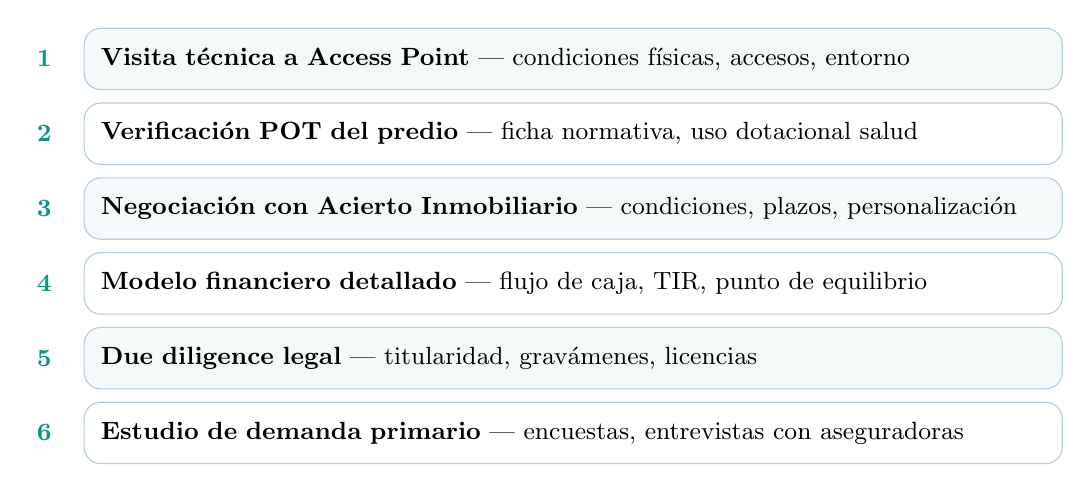
\begin{tikzpicture}[
  stepbox/.style={draw=hptu!30, fill=white, rounded corners=6pt,
              text width=12cm, minimum height=0.78cm, align=left,
              font=\small, inner sep=6pt},
  num/.style={font=\small\bfseries, teal, anchor=east},
]
\node[stepbox, fill=teal!5] (s1) at (0,0) {
  \textbf{Visita técnica a Access Point} --- condiciones físicas, accesos, entorno
};
\node[num] at (-6.5,0) {1};

\node[stepbox] (s2) at (0,-0.95) {
  \textbf{Verificación POT del predio} --- ficha normativa, uso dotacional salud
};
\node[num] at (-6.5,-0.95) {2};

\node[stepbox, fill=teal!5] (s3) at (0,-1.9) {
  \textbf{Negociación con Acierto Inmobiliario} --- condiciones, plazos, personalización
};
\node[num] at (-6.5,-1.9) {3};

\node[stepbox] (s4) at (0,-2.85) {
  \textbf{Modelo financiero detallado} --- flujo de caja, TIR, punto de equilibrio
};
\node[num] at (-6.5,-2.85) {4};

\node[stepbox, fill=teal!5] (s5) at (0,-3.8) {
  \textbf{Due diligence legal} --- titularidad, gravámenes, licencias
};
\node[num] at (-6.5,-3.8) {5};

\node[stepbox] (s6) at (0,-4.75) {
  \textbf{Estudio de demanda primario} --- encuestas, entrevistas con aseguradoras
};
\node[num] at (-6.5,-4.75) {6};
\end{tikzpicture}
\end{center}

\vspace{4pt}
{\footnotesize\textcolor{slate}{Timeline estimado: pasos 1-3 en abril, pasos 4-6 en mayo-junio.}}
\end{frame}

% ---- SLIDE 28: SINTESIS ----
{
\setbeamercolor{background canvas}{bg=teal!4}
\begin{frame}{Síntesis: por qué Access Point, por qué ambulatorio}
\vspace{-2pt}
\begin{center}
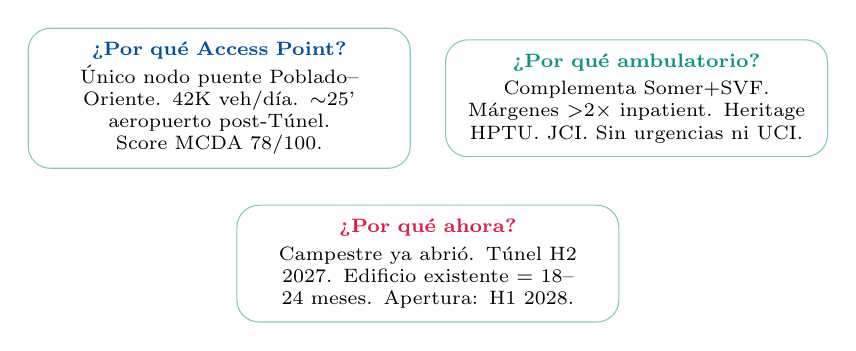
\begin{tikzpicture}[
  box/.style={draw=teal!50, fill=white, rounded corners=8pt,
              text width=4.5cm, minimum height=1.4cm, align=center,
              font=\scriptsize, inner sep=5pt},
]
\node[box] (why) at (0,0) {
  \textcolor{hptu}{\textbf{¿Por qué Access Point?}}\\[2pt]
  Único nodo puente Poblado--Oriente.
  42K veh/día. $\sim$25' aeropuerto post-Túnel.
  Score MCDA 78/100.
};

\node[box] (what) at (5.3,0) {
  \textcolor{teal}{\textbf{¿Por qué ambulatorio?}}\\[2pt]
  Complementa Somer+SVF.
  Márgenes $>$2$\times$ inpatient.
  Heritage HPTU. JCI.
  Sin urgencias ni UCI.
};

\node[box] (when) at (2.65,-2.1) {
  \textcolor{rose}{\textbf{¿Por qué ahora?}}\\[2pt]
  Campestre ya abrió. Túnel H2 2027.
  Edificio existente = 18--24 meses.
  Apertura: H1 2028.
};
\end{tikzpicture}
\end{center}

\vspace{2pt}
\begin{exampleblock}{}
\centering
\highlight{Recomendación: sede ambulatoria HPTU en Access Point, Km 7 Vía Las Palmas}
\end{exampleblock}

\vspace{1pt}
{\tiny\textbf{¿Por qué no El Poblado?} Ya tiene Torre Oviedo, Rosario Tesoro, CEDIMED, BlueCare. Competencia ambulatoria \danger{densa}. AP captura \highlight{ambos mercados}: Poblado + 298K Oriente.}
\end{frame}
}

% ---- SLIDE 29: CIERRE ----
{
\setbeamercolor{background canvas}{bg=hptu}
\begin{frame}[plain]
\vfill
\begin{center}
{\Huge\bfseries\textcolor{white}{Plan de Expansión HPTU}}

\vspace{12pt}
{\Large\textcolor{white!85}{Sede Ambulatoria en Access Point}}

\vspace{20pt}
\begin{tikzpicture}
  \draw[white, line width=0.5pt] (0,0) -- (6,0);
\end{tikzpicture}

\vspace{14pt}
{\normalsize\textcolor{white!70}{MCDA 78/100 $\cdot$ 5 dimensiones $\cdot$ 6 escenarios Monte Carlo}}

\vspace{6pt}
{\normalsize\textcolor{white!70}{Apertura estimada: H1 2028 $\cdot$ CAPEX: COP \$67,000M}}

\vspace{6pt}
{\normalsize\textcolor{white!70}{Revenue: \$51,000M $\cdot$ EBITDA: \$9,200M $\cdot$ Payback: 6--8 años}}

\vspace{20pt}
{\small\textcolor{white!50}{Dashboard: hptu-localizacion.vercel.app}}

\vspace{14pt}
{\footnotesize\textcolor{white!50}{Abril 2026}}
\end{center}
\begin{tikzpicture}[remember picture, overlay]
  \node[anchor=south]
    at ([yshift=14pt]current page.south) {
    
\includegraphics[height=1.2cm]{basica-white.png}
  };
\end{tikzpicture}
\vfill
\end{frame}
}

\end{document}
